\documentclass[a4paper,14pt]{extarticle}

% Russian-specific packeges
%--------------------------------
\usepackage[T2A]{fontenc}
\usepackage[utf8]{inputenc}
\usepackage[russian]{babel}
%--------------------------------
\usepackage{csquotes}
\usepackage{hyphenat}
\usepackage{subcaption}

\usepackage{biblatex} %Imports biblatex package
\addbibresource{ref.bib} %Import the bibliography file

\usepackage{amsmath,amssymb}
\usepackage{indentfirst}
\usepackage{graphicx}
\usepackage{hyperref}

\usepackage[left=3cm, right=1.5cm, top=2cm, bottom=2cm]{geometry} % Меняем поля страницы

\graphicspath{ {diploma_pictures} }

\usepackage{physics}

\linespread{1.3}



\begin{document}
    \thispagestyle{empty}
    \begin{titlepage}
    \small
    \begin{center}
    ФЕДЕРАЛЬНОЕ ГОСУДАРСТВЕННОЕ БЮДЖЕТНОЕ ОБРАЗОВАТЕЛЬНОЕ
    УЧРЕЖДЕНИЕ ВЫСШЕГО ОБРАЗОВАНИЯ \\
    «МОСКОВСКИЙ ГОСУДАРСТВЕННЫЙ УНИВЕРСИТЕТ\\
    имени М.В. ЛОМОНОСОВА»
    \vspace{0.5cm}

    ФИЗИЧЕСКИЙ ФАКУЛЬТЕТ\\
    \vspace{0.5cm}
    КАФЕДРА КВАНТОВОЙ ТЕОРИИ И ФИЗИКИ ВЫСОКИХ ЭНЕРГИЙ\\

    \vspace{0.5cm}
    БАКАЛАВРСКАЯ РАБОТА \\
    \vspace{3cm}

    \textbf{<<Поиск возможностей повышения чувствительности экспериментального исследования спектра бета-распада молекулярного трития к оценке эффективной массы электронного антинейтрино.>>}


    \end{center}


    \begin{flushright}
    \vspace{3cm}

    Выполнил студент \\
    408 группы\\

    Зубрилин Кирилл Васильевич \\

    \underline{\hspace{3cm}}\\

    \vspace{0.5cm}

    Научный руководитель:\\
    д.ф.\--м.н. Свешников Константин Алексеевич \\
    \underline{\hspace{3cm}}\\
     
    \vspace{0.5cm}

    Научный консультант:\\
    к.ф.\--м.н. Титов Никита Андреевич \\
    
    \end{flushright}

    %\vspace{1cm}
    \begin{flushleft}
    Допущена к защите \\
    Зав. кафедрой \underline{\hspace{3cm}} \\
    \end{flushleft}
    \begin{center}
    \vspace{1.5cm}
    \small МОСКВА \\ \number\year\normalsize
    \end{center}
    \end{titlepage}

    \tableofcontents
    \setcounter{page}{2}
    \newpage
    \section{Введение}

    %===========================================================================================
    Нейтрино являются весьма особенными для науки частицами, которые снова и снова 
    приводили к неожиданным и невероятным открытиям, ряд из которых отмечен Нобелевскими 
    премиями. Нейтрино были теоретически введены в 1930 году Паули для выполнения закона сохранения 
    энергии-импульса, а их первое экспериментальное обнаружение состоялось в 1956 году 
    группой Рейнеса и Коуэна на реакторе электростанции Savannah River. Позже оказалось, что существует три аромата нейтрино,
    что снова стало важным открытием. Затем были зарегистрированы осцилляции солнечных 
    нейтрино по пути их распространения к Земле, что является квантовомеханическим эффектом,
    обычно проявляющимся лишь в атомных масштабах. Было обнаружено, что нейтрино имеют 
    очень маленькую массу, что до сих пор является единственным значимым свидетельством
    существования физики элементарных частиц за пределами Стандартной модели. Есть множество других областей, где уже признано, 
    что нейтрино играют важную роль, но есть очень серьезные поводы полагать, что в будущем 
    могут появиться еще более удивительные результаты. Нейтрино — это безмассовые частицы в 
    Стандартной модели. Прямое расширение СМ для введения масс нейтрино, аналогичных массам 
    заряженных лептонов, заключается в добавлении правых (синглетных) нейтринных полей; в этом 
    случае  взаимодействия Юкавы будут свидетельствовать о наличии дираковских масс нейтрино 
    после нарушения электрослабой симметрии. Однако это предположение не считается удовлетворительным 
    сообществом теории нейтрино по двум причинам: а) не объясняет, почему абсолютная шкала 
    массы нейтрино по крайней мере в миллион раз меньше, чем массы других фермионов СМ, и 
    б) симметрии СМ не запрещают другие, так называемые Массовые члены Майораны для недавно 
    введенных правых полей нейтрино. Эти массы не ограничены сверху средним значением вакуума 
    Хиггса и, следовательно, должны принимать много большие значения, чем масса t-кварка. 
    Принимая во внимание массовые члены Майораны, мы получим эффективные массы легких майорановских 
    нейтрино в абсолютной шкале масс нейтрино $m_{\nu} \simeq m^2_D/M_R$; здесь $m_{D}$ и $M_R \geq 10^{14}$ ГэВ 
    величины электрослабого нарушения симметрии и тяжелых майорановских нейтрино соотвественно. 
    Этот механизм установлен как механизм качелей типа I (<<see-saw mechanism>>) \cite{minkowski} 
    \cite{https://doi.org/10.48550/arxiv.1306.4669}; это интересно, так как дает описание 
    малости массы нейтрино, имеет потенциальную связь с лептогенезом и может даже подразумевать 
    отношение к шкале, объединяющей электрослабое и сильное взаимодействия. Тогда массы легких 
    нейтрино появляются как собственные значения массовой матрицы Майорана, а матрица 
    Понтекорво-Маки-Накагава-Саката (далее ПМНС) U получается из относительного вращения полей 
    левых заряженных лептонов и нейтрино (с которыми связан заряженный ток).
    
    Вспомним, что абсолютные массы нейтрино появляются в теории как собственные состояния матрицы 
    эффективных масс легких нейтрино. Хотя эксперименты с нейтринными осцилляциями способны измерять 
    расщепление квадрата массы среди них и даже упорядочение масс, они не могут дать абсолютную 
    шкалу масс нейтрино. Осцилляции нейтрино дают нижнюю оценку суммы масс нейтрино 0,06 эВ и 0,10 эВ 
    для нормального и обратного порядков соответственно, в то время как текущие верхние границы, полученные 
    различными методами, $\simeq$ 1 эВ. Если сумма масс нейтрино близка к нижней границе, мы говорим 
    об иерархической схеме, где масса легкого нейтрино ближе к нулю по сравнению с расщеплениями масс. 
    Если она близка к верхней границе, то речь уже идет о вырожденных массах нейтрино, поскольку расщепления 
    $|\Delta m^2| \ll m^2 $ малы по сравнению с массами. Порядок масс нейтрино и масштаб шкалы являются
    важными параметрами для теоретических моделей, потому что устройство аромата в лагранжиане, описывающем 
    массу нейтрино будет сильно различаться в нормальном иерархическом, обратном иерархическом и вырожденном случаях. 
    
    В значительной степени независимым способом получить абсолютную шкалу масс нейтрино 
    являются точные кинематические эксперименты по изучению слабых взаимодействий. Сегодня 
    основные усилия направлены на исследовании двух процессов: бета-распада трития ($^{3}$H) и 
    захват электрона гольмием ($^{163}$Ho). Что интересно, данные методы позволяют независимо 
    получить массы электронных нейтрино и антинейтрино, которые должны быть равны при CPT 
    инвариантности. Особенность данных методов состоит в том, что напрямую измеряются квадраты
    масс нейтрино, что приводит к некоторым трудностям при получении оценки непосредственно массы нейтрино. 
    
    Для тритиевых экспериментов используются электростатические спектрометры с адиабатической магнитной коллимацией (так называемые MAC-E фильтры) \cite{lobashev} \cite{picard}.
    Проект КАТРИН в максимальной степени использует данную технологию, что на сегодняшний день позволило
    получить значение верхней границы массы нейтрино 0.8 эВ (при 90\% доверительном уровне) \cite{aker}.
    КАТРИН продолжит набор статистики для достижения проектной чувствительности на уровне 0.2 эВ.
    
    
    Актуальность проекта «КАТРИН» подтверждается  
    тем, что публикации по теме проекта набрали более 800 ссылок
    в высокорейтинговых изданиях за последние два года.

    Данная работа выполнена в рамках проекта КАТРИН, в ней исследуются способы повышения 
    чувствительности эксперимента к массе электронного антинейтрино. 
    
     

    %===========================================================================================


    %===========================================================================================
    \newpage
    \section{Обзор задачи}
    \subsection{Устройство спектрометра}
    Высокая чувствительность экспериментов по массе нейтрино в Троицке и Майнце обусловлена
    новым типом спектрометра, так называемым MAC-E фильтром (электростатическим фильтром с адиабатической магнитной коллимацией). 
    +. Впервые этот новый тип спектрометра был предложен
    в \cite{Beamson_1980}. Позднее этот метод был переизобретен специально для поиска массы электронного
    антинейтрино независимо друг от друга в Троицке и Майнце \cite{lobashev} \cite{picard}. Разрешение такого спектрометра определяется адиабатичностью движения электронов в медленно меняющихся электрических и магнитных полях и не зависит от размеров источника. Поэтому он сочетает в 
    себе высокие светимость и энергетическое разрешение, необходимые для измерения массы нейтрино в области конца спектра $\beta$-распада. Одновременно магнитное поле изолирует поток электронов из распада в объеме безоконного газового источника от электронов из распада трития адсорбированного на стенках и электронов испытавших рассеяние на элементах конструкции.  
    
    Принцип действия MAC-E-фильтра показан на рис. \ref{fig:spectrometer}(a) \cite{design_report}. 
    Два сверхпроводящих соленоида создают направляющее магнитное поле. Электроны, рождаемые в источнике
    трития, находящемся в левом соленоиде, вылетают в направлении на спектрометр, при этом их отклонение от силовой линии ведущего магнитного поля определяется радиусом циклотронного движения для текущего значения величины магнитного поля, что позволяет рассчитать степень их изоляции  
    от электронов рожденных вне трубки магнитного поля. Величина магнитного поля $B$ на пути в центр спектрометра падает на несколько порядков. 
В медленно меняющихся полях величина первого адиабатического инварианта - магнитного момента $\mu$ остается постоянной:
    
    \begin{equation}\label{adiabat}
        \mu = \frac{E_\perp}{B} = const.
    \end{equation}

Это приводит к преобразованию большей части энергии поперечного движения в продольную. Вращение вектора импульса 
    показано на рис. \ref{fig:spectrometer}(б). Проявление адиабатичности движения можно резюмировать следующим образом: электроны, изотропно испускаемые
    источником, преобразуются в широкий пучок электронов, летящих почти параллельно линиям магнитного поля. 
В центральной области продольная компонента энергии электронов анализируется электрическим запирающим потенциалом. Ширина переходной области электростатического анализатора определяется конечной степенью «выстроенности» электронов в анализирующей плоскости. 
    
    \begin{figure}
        \center
        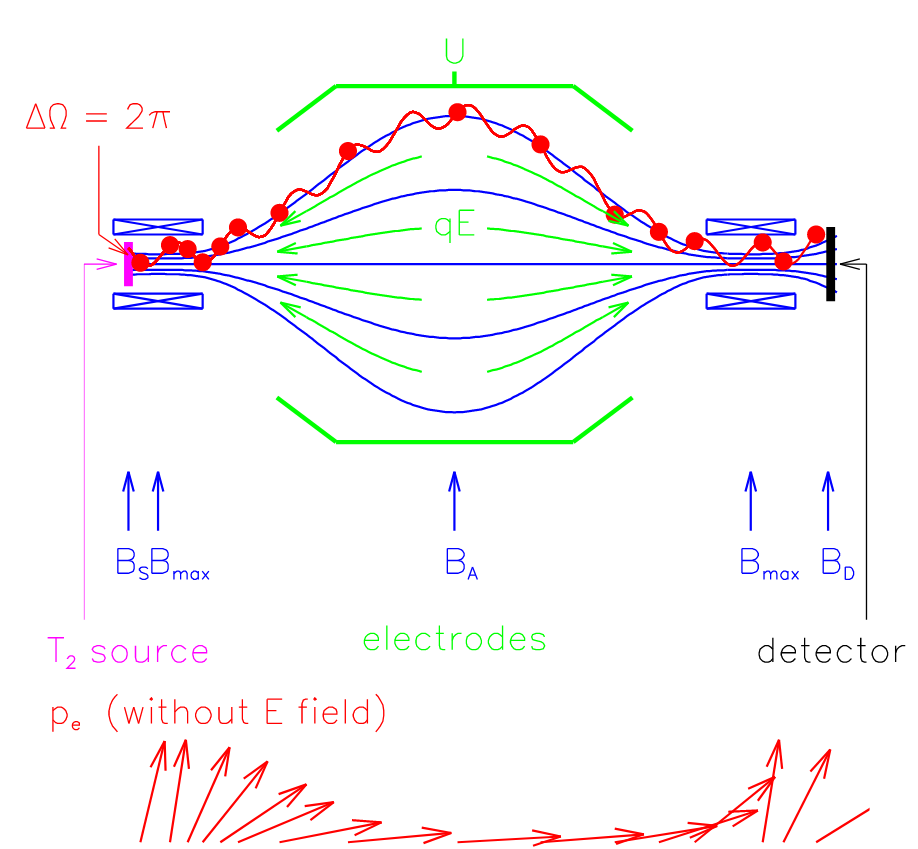
\includegraphics[width=0.6\textwidth]{spectrometer.png}
        \captionsetup{width=0.8\textwidth}
        \caption{Принципиальная схема MAC-E фильтра. (а) Экспериментальная установка, (б) Преобразование вектора импульса, обусловленное сохранением адиабатического инварианта $\mu$.}
        \label{fig:spectrometer}
    \end{figure}
    
    Получившийся параллельный пучок электронов летит против градиента электростатического потенциала, образованного
    одним или несколькими цилиндрическими электродами. Все электроны с энергией, достаточной для прохождения
    электростатического барьера, вновь ускоряются и коллимируются на детекторе, остальные же отражаются.
    Таким образом спектрометр действует как фильтр электронов низких энергий. Из уравнения (\ref{adiabat})
    непосредственно следует, что относительная резкость $\Delta E/E$ этого фильтра определяется только соотношением
    минимального магнитного поля $B_A$ в центральной плоскости и максимального магнитного поля
    $B_{max}$ между источником электронов и спектрометром:
    
    \begin{equation}
        \label{form2}
        \frac{\Delta E}{E} = \frac{B_A}{B_{max}}
    \end{equation}
    
    Чтобы подавить электроны, которые имеют очень длинный путь внутри источника трития
    и, следовательно, обладают высокой вероятностью рассеяния, источник электронов помещается в
    магнитное поле $B_S$, которое меньше максимального магнитного поля $B_{max}$.
    Это ограничивает максимально допустимый начальный угол электронов $\theta_{max}$:
    электроны с углами $\theta > \theta_{max}$ отражаются от магнитного поля $B_{max}$.
    
    \begin{equation}
        \label{form3}
        \sin \theta_{max} = \sqrt{\frac{B_S}{B_{max}}}.
    \end{equation}
    
    Из ур. (\ref{adiabat}), (\ref{form2}) и (\ref{form3}) следует, что нормированная функция пропускания MAC-E
    фильтра с задерживающим потенциалом U для изотропного источника электронов с энергией $E$ дается выражением:
    
    \begin{equation}
    \begin{split}
      T(E,U) = \int_{0}^{\theta_{max}} \mathcal T(E, \theta, U) \sin\theta\cdot d\theta = \\
      \begin{cases} 
        0 & , E - qU < 0 \\
        \frac{1 - \sqrt{1-\frac{E-qU}{E} \frac{B_{S}}{B_{A}}}}{1 - \sqrt{1-\frac{\Delta E}{E}\frac{B_{S}}{B_{A}}}} & , 0 \leq E-qU \leq \Delta E \\
        1 & , E - qU > \Delta E
      \end{cases}
    \end{split}
    \end{equation}
    
    \noindent где $q$ - заряд электрона, а $\mathcal T(E, \theta, U)$ равна: 
    
    \begin{equation}
      \mathcal T(E, \theta, U) = 
      \begin{cases}
        1 & , E(1-\sin^2 \theta \cdot \frac{B_{min}}{B_S}) -qU > 0 \\
        0 & , E(1-\sin^2 \theta \cdot \frac{B_{min}}{B_S}) -qU \leq 0
      \end{cases}
    \end{equation}
    
    
    \subsection{Расчет спектра}
    Для определения массы нейтрино необходимо сопоставить экспериментальные данные
    с теоретическим предсказанием, полученным с помощью аналитической формулы $\beta$-распада
    и экспериментальной функции отклика, описанными ниже.
    
    Дифференциальный спектр $\beta$-распада берется из теории Ферми и описывается
    формулой:
    
    \begin{equation}
      \begin{split}
        R_{\beta}(E) = \frac{G_F^2 \cos^2 \Theta_C}{2 \pi^3} |M_{nucl}|^2 F(E, Z'=2) \cdot \\
        (E + m_e) \sqrt{(E+m_e)^2-m_e^2} \cdot \\
        \displaystyle\sum_f \zeta_f \varepsilon_f(E) \sqrt{\varepsilon_f(E)^2-m_{\nu}^2} \cdot \Theta(\varepsilon_f(E)-m_{\nu}),
      \end{split}
    \end{equation}
    
    \noindent где $G_F$ - константа Ферми, $\cos^2 \Theta_C$ - угол Кабиббо, $|M_{nucl}|^2$ - независящий от энергии для распада трития матричный
    элемент, а $F(E, Z'=2)$ - функция Ферми. $\varepsilon_f(E) = E_0 - V_f - E$, где $E_0$ - максимальная кинетическая
    энергия электрона для безмассового нейтрино, $V_f$ и $\zeta_f$ описывают спектр возбужденных состояний при распаде
    трития в состояние дочернего молекулярного иона $(^3HeT^+)^*$ с энергией возбуждения $V_f$, которые распределены с
    вероятностями $\zeta_f$ (спектр возбужденных состояний получается расчетным путем и входит в список 
    систематических погрешностей), $E$ и $m_e$ - кинетическая энергия и масса электрона соответственно.
    
    Теоретический спектр $R(qU,r)$ задается суммой свёртки дифференциального спектра $\beta$-распада $R_{\beta}(E)$ 
    с экспериментальной функцией отклика $f(E,qU,R)$ и фона $R_{bg}(qU,r)$:
    \begin{equation}
      R(qU,r)=N_T \int_{qU}^{E_0} R_{\beta}(E)f(E,qU,R)dE + R_{bg}(qU,r).
    \end{equation}
    
    Здесь $N_T$ - нормировочная константа сигнала, зависящая от числа атомов трития в источнике, максимального угла
    раскрытия, потерь электронами энергии за счет неупругого рассеяния в источнике и других параметров
    экспериментальной установки. 
    
    \begin{figure}
        \center
        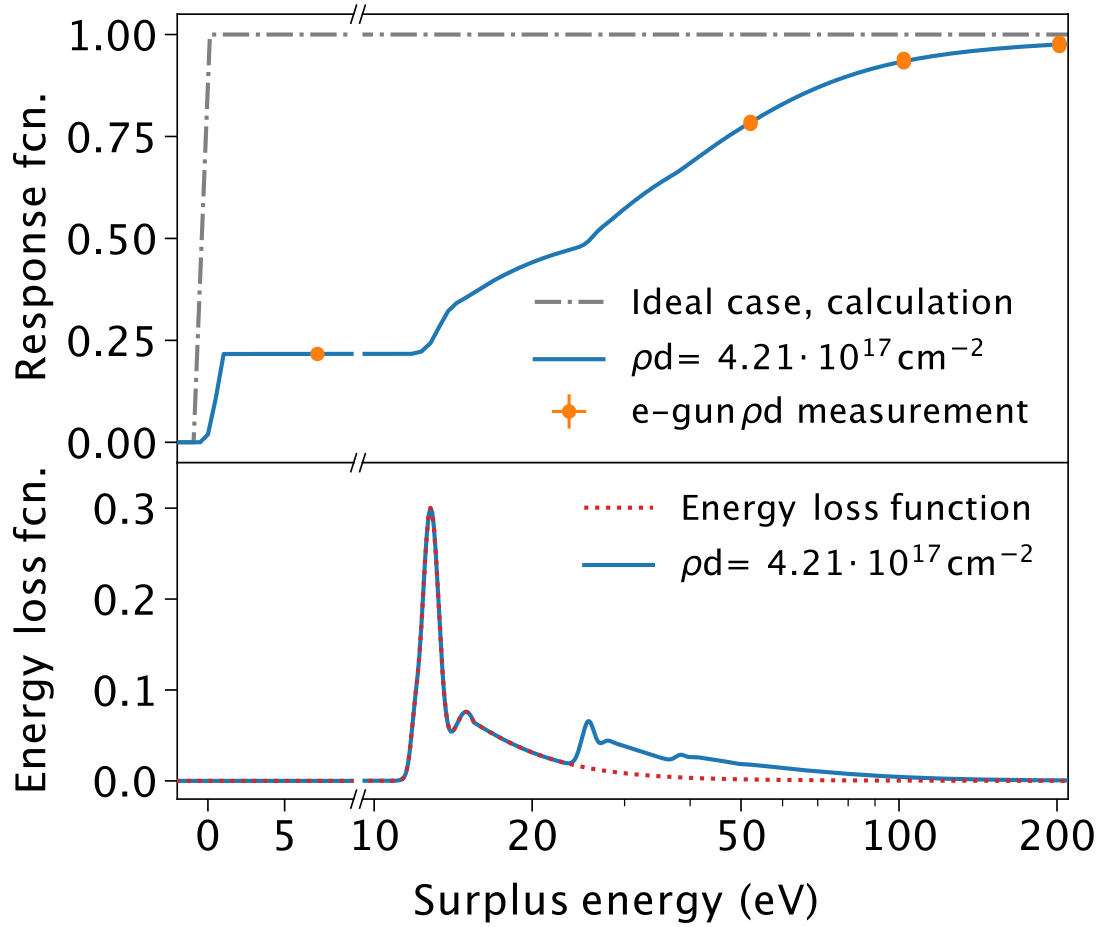
\includegraphics[width=0.6\textwidth]{response.png}
        \captionsetup{width=0.8\textwidth}
        \caption{Функции отклика и энергетических потерь спектрометра.}
        \label{fig:response}
    \end{figure}
    
    Экспериментальная функция отклика (рис. \ref{fig:response} \cite{katrin_status})
    
    \begin{equation}
      f(E-qU) = \int_0^{E-qU} \int_0^{\theta_{max}} \mathcal T(E - \varepsilon, \theta, U) \sin\theta \\
      \cdot \displaystyle\sum_s P_s(\theta)f_s(\varepsilon) d\theta d\varepsilon
    \end{equation}
    
    \noindent выражает вероятноять электрона с начальной энергией $E$ достигнуть детектора. Она содержит функцию 
    пропускания спектрометра $\mathcal T(E - \varepsilon, \theta, U)$ и энергетические потери электрона
    $\varepsilon$, вызванные неупругими столкновениями с молекулами трития в источнике. Потери энергии, вызванные
    рассеянием, описываются как произведение вероятности s-кратного рассеяния $P_s(\theta)$, которая зависит от пути 
    пройденного через источник и, как следствие, угла падения $\theta$, и функции энергетических потерь 
    $f_s(\varepsilon)$ для числа рассеяний s. Функция потерь определяется экспериментально с помощью электронной
    пушки, установленной у входа в источник.
    
    
    
    
    \subsection{Критерий Колмогорова-Смирнова}
    Для проверки того, порождена ли выборка случайной величиной $\xi$ с функцией распределения $F(x)$, необходимо 
    построить эмпирическую функцию распределения $F_n(x)$:
    
    \begin{equation}
      F_n(x) = \frac{1}{n} \sum_{i=1}^n I_{X_i \leq x},
    \end{equation}
    
    \noindent где $I_{X_i \leq x}$ - индикаторная функция.
    
    \begin{equation}
      I_{X_i \leq x} = 
      \begin{cases}
        1, & X_i \leq x; \\
        0, & X_i > x.
      \end{cases}
    \end{equation}
    
    Далее вычисляется статистика Колмогорова-Смирнова \cite{kolmogorov} \cite{frank_j}, которая равна 
    максимальному модулю разности между двумя распределениями:
    
    \begin{equation}
      D_n = \sup_x |F_n(x) - F(x)|.
    \end{equation}
    
    Тесту подвергается нулевая гипотеза $H_0$ о том, что исследуемая выборка подчиняется распределению
    $F(x) \in C^1$. По теореме Колмогорова для введенной ранее статистики справедливо:
    
    \begin{equation}
      \lim_{n \rightarrow \infty} P(\sqrt{n}D_n \leq y) = K(y),
    \end{equation}
    
    \noindent где $K(y)$ - функция распределения Колмогорова (рис. \ref{fig:kolmogorov}) равная:
    \begin{equation}
      K(y) = \sum_{j=-\infty}^{+\infty} (-1)^j\exp^{-2j^2y^2}, y > 0.
    \end{equation}
    
    \begin{figure}
        \center
        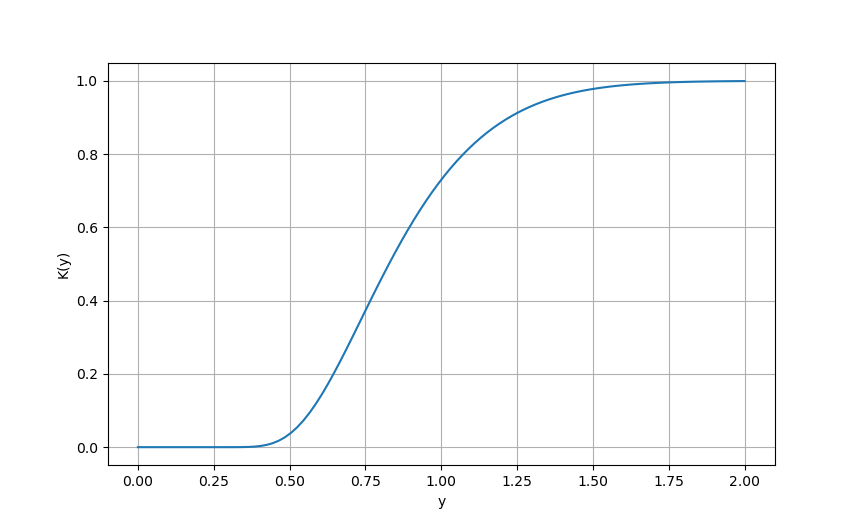
\includegraphics[width=0.9\textwidth]{kolmogorov.png}
        \captionsetup{width=0.8\textwidth}
        \caption{Функция распределения Колмогорова.}
        \label{fig:kolmogorov}
    \end{figure}
    
    Тогда мы отвергаем гипотезу о совпадении распределений с уровнем доверия $\alpha$, если
    
    \begin{equation}
      \sqrt{n}D_n > K_{\alpha},
    \end{equation}
    
    \noindent где $K_{\alpha}$ находится из условия

    \begin{equation}
      P(K \leq K_{\alpha}) = 1 - \alpha.
    \end{equation}
    
    В данной же работе применяется модифицированный критерий Кол- могорова-Смирнова -- 
    критерий Лиллиефорса\cite{lilliefors}. Он используется для проверки гипотезы о том, что
    выборка принадлежит нормальному распределению. Его особенность заключается в том, что
    априори параметры распределения неизвестны и находятся как выборочное среднее и дисперсия.
    
    Однако необходимо учитывать факт, что параметры оцениваются по тем же самым данным, которые
    проверяются на соответствие распределению. В этом случае значение статистики будет меньше,
    чем в случае, когда параметры распределения получены независимо. Поэтому распределение, 
    на основании которого принимается решение об истинности гипотезы, смещено в сторону меньших
    значений относительно распределения Колмогорова и известно как распределения Лиллиефорса и
    рассчитывается методом Монте-Карло.
    
    
    %\subsection{Критерий Андерсона-Дарлинга}

    %===========================================================================================
    
    \newpage
    \section{Основная часть}
    
    \subsection{Учет отрицательных $m_{\nu}^2$}
    
    \begin{figure}[h]
        \center
        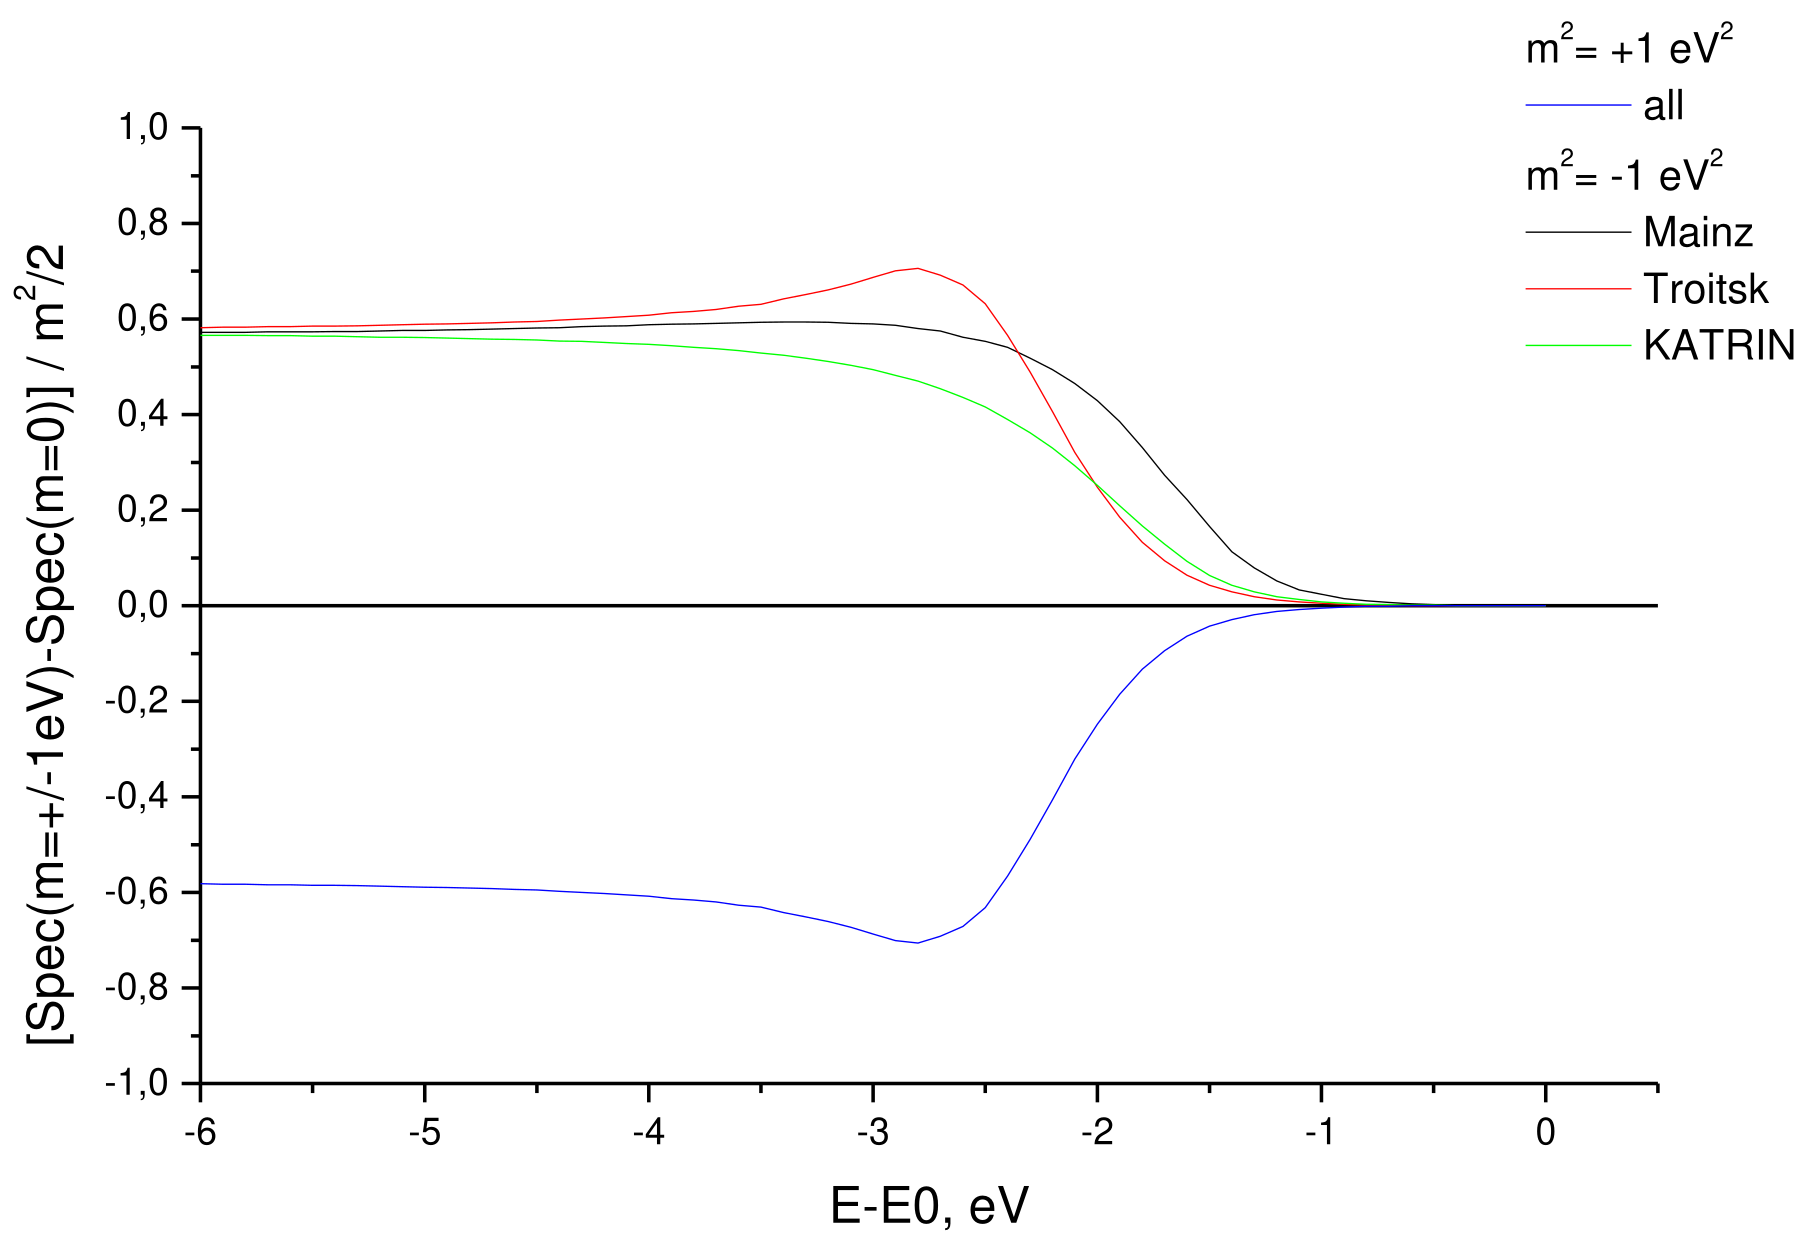
\includegraphics[width=0.9\textwidth]{neg_mnu2.png}
        \captionsetup{width=0.8\textwidth}
        \caption{Форма спектра при отрицательном квадрате массы нейтрино.}
        \label{fig:neg_mnu2}
    \end{figure}
    
    Из-за статистической природы измерений при фитировании экспериментальных данных мы можем
    получить как положительные, так и отрицательные значения квадрата массы антинейтрино.
    
    В Троицке учет отрицательного квадрата массы нейтрино дается следующей формулой:
    
    \begin{equation}
      \text{Sp}(E, m^2_\nu<0) = \text{Sp}(E, m^2_\nu=0) + [\text{Sp}(E, m^2_\nu=0) - \text{Sp}(E, |m^2_\nu|)]
    \end{equation}
    
    При анализе данных эксперимента в Майнце\cite{kraus} теоретическая формула спектра при фитировании
    модифицировалась так, чтобы $\chi^2$ представлял собой параболу вблизи значения $m_\nu^2 = 0$.
    Это достигалась введением фактора $g_f$ для каждого электронного состояния в формуле
    
    \begin{equation}
    \begin{split}
      g_f = \Theta(-m_\nu^2)\Theta(\varepsilon_f+\mu)(1+\frac{\mu}{\varepsilon_f}\exp^{-(1+\varepsilon_f/\mu)}) \\
      +\Theta(m_\nu^2)\Theta(\varepsilon_f-m_\nu^2)
    \end{split}
    \end{equation}
    
    \noindent где $\mu = -0.66 m^2_\nu c^4$. Для отрицательных значений квадрата массы граничная
    энергия сдвигается к значению $E_0-V_f+\mu$, <<растягивая>> спектр.
    
    В КАТРИН процедура фита проходит без особого учета отрицательного квадрата массы.
    
    На рис. \ref{fig:neg_mnu2} изображены формы спектры при отрицательном квадрате массы
    для описанных случаев.
    
    
    
\subsection{Асимметрия распределения (skewness)}

%Отклонение распределения результатов анализа экспериментов типа «КАТРИН» от распределения  Гаусса проявляется в появлении у него асимметрии (skewness).

%Асимметрия распределения связана с необходимостью выбора продолжения формы экспериментального спектра на область отрицательного квадрата массы нейтрино. Последнее связано с тем, что фазовый объем нейтрино в области е^2 >> m^2 сводится к величине е^2 – 1/2 m^2 и для определения квадрата массы необходимо сравнить величину скорости счета в точке экстраполированного конца спектра с скоростью счета фона. Обе величины подвержены флуктуациям и их разность может принимать как положительные, так и отрицательные значения. Если один знак разности интерпретируется как сигнал ненулевой массы нейтрино, то противоположный является нефизическим. Тем не менее его нужно правильно интерпретировать с тем, чтобы оценка массы нейтрино из экспериментальных данных была несмещенной.     

  
  \subsection{Влияние величины статистики на результат}
    
    
    Одной из проблем, с которой столкнулись при проведении эксперимента КАТРИН, оказался медленный дрейф
    потенциала газового источника, связанная с изменением работы выхода материала источника за счет
    его взаимодействия с компонентами газовой смеси. Для минимизации данного эффекта рассматривается
    возможность разбиения экспериментальных данных на короткие по времени подгруппы.
    
    Для этого на языке Python была написана программа, вычисляющая спектр c $m^2_\nu=0$ 
    в соответствии с описанием, приведенным в обзоре задачи. Вычисление проводится с 
    использованием интерполяции на основе предрассчитанных данных, это позволяет
    производить вычисления на обычном персональном компьютере за сравнительно 
    небольшие промежутки времени. Для точек расчитанного
    спектра вносятся ошибки пропорциональные экспериментальным ошибкам в ходе проведения 
    первой серии измерений на КАТРИН (KNM1) -- $\Delta R_{exp} \cdot \xi$, где $\xi$ -
    случайная величина $\in N(0, \sigma^2_{err} = 1)$. Далее производится фитирование полученного
    спектра методом минимизации $\chi^2$ с помощью модуля iminuit, основанного на известной
    библиотеке для языков FORTRAN и C. Рассматривается три описанных выше случая учета
    в формуле отрицательного квадрата массы нейтрино.
    
    
    \begin{figure}
        \center
        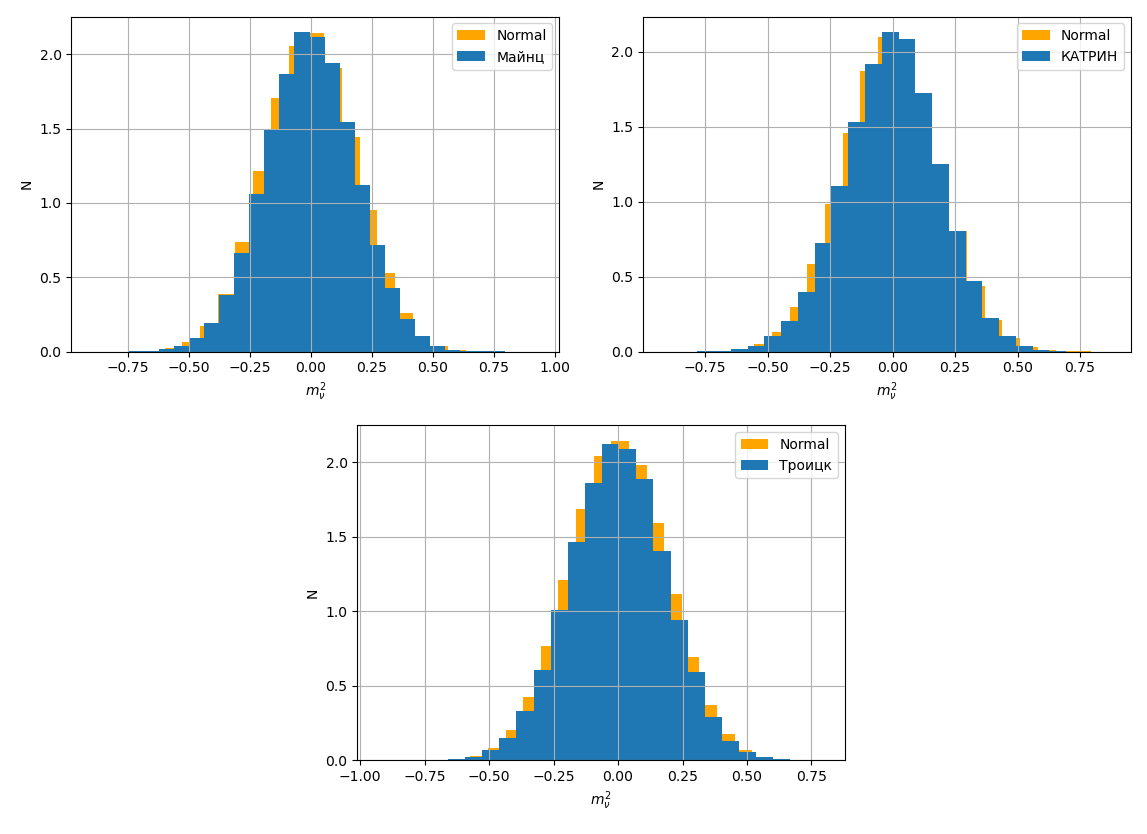
\includegraphics[width=0.9\textwidth]{hists}
        \captionsetup{width=0.8\textwidth}
        \caption{Результаты для разных формул.}
        \label{fig:hists}
    \end{figure}
    
    \begin{table}
      \caption{Результаты фита для разного числа прогонов и формул.}
	    \begin{center}
		    \begin{tabular}{|r|r|r|r|r|r|r|}
			    \hline
			    Formula & N & $m^2_\nu$ & $\sigma$ & $D_n$ & $\alpha$ & skew \\
			    \hline
			    mainz & 1000 & -2.86e-03e & 0.190 & 0.02742 & 0.432 & 0.0649 \\
			    \hline
			    mainz & 10000 & -7.77e-04e & 0.186 & 0.00718 & 0.678 & -0.0108 \\
			    \hline
			    mainz & 100000 & -9.66e-05e & 0.184 & 0.00231 & 0.658 & -0.0120 \\
			    \hline
			    katrin & 1000 & 4.23e-03e & 0.187 & 0.02255 & 0.680 & -0.0453 \\
			    \hline
			    katrin & 10000 & -1.76e-03e & 0.190 & 0.00989 & 0.280 & -0.0681 \\
			    \hline
			    katrin & 100000 & -1.99e-03e & 0.188 & 0.00732 & 0.000 & -0.0643 \\
			    \hline
			    troitsk & 1000 & -3.46e-03e & 0.186 & 0.01386 & 0.989 & 0.1140 \\
			    \hline
			    troitsk & 10000 & 1.70e-03e & 0.186 & 0.00626 & 0.825 & 0.0273 \\
			    \hline
			    troitsk & 100000 & 8.32e-04e & 0.185 & 0.00231 & 0.657 & -0.0080 \\
			    \hline
		    \end{tabular}
	    \end{center}
    \end{table}
    
    Для случаев Майнца и КАТРИН проводится тест с различными значениями $\sigma$, что соответствует
    различному времени набора статистики.
      
	  \begin{table}
	    \caption{Результаты для формулы КАТРИН с различными значениями разброса ошибки.}
	    \begin{center}
		    \begin{tabular}{|r|r|r|r|r|r|r|}
			    \hline
			    $\sigma_{err}$ & N & $m^2_\nu$ & $\sigma$ & $D_n$ & $\alpha$ & skew \\
			    \hline
			    0.1 & 100000 & 5.36e-04 & 0.019 & 0.00219 & 0.720 & -0.0093 \\
			    \hline
			    0.2 & 100000 & 4.57e-04 & 0.037 & 0.00187 & 0.873 & -0.0151 \\
			    \hline
			    0.25 & 100000 & 5.91e-04 & 0.047 & 0.00316 & 0.270 & -0.0393 \\
			    \hline
			    0.4 & 100000 & 1.75e-04 & 0.075 & 0.00396 & 0.087 & -0.0435 \\
			    \hline
			    0.5 & 100000 & 4.59e-05 & 0.093 & 0.00561 & 0.004 & -0.0485 \\
			    \hline
			    1 & 100000 & -1.99e-03 & 0.188 & 0.00732 & 4.5e-05 & -0.0643 \\
			    \hline
			    2 & 100000 & -8.30e-03 & 0.382 & 0.01035 & 9.8e-10 & -0.1067 \\
			    \hline
			    4 & 100000 & -2.46e-02 & 0.775 & 0.01391 & 3.1e-17 & -0.1458 \\
			    \hline
		    \end{tabular}
	    \end{center}
    \end{table}
    
    \begin{table}
	    \begin{center}
	      \caption{Результаты для формулы Майнца с различными значениями разброса ошибки.}
		    \begin{tabular}{|r|r|r|r|r|r|r|}
		    	\hline
		      $\sigma_{err}$ & N & $m^2_\nu$ & $\sigma$ & $D_n$ & $\alpha$ & skew \\
		      \hline
		      0.1 & 100000 & 6.40e-04 & 0.018 & 0.00158 & 0.963 & -0.0021 \\
		      \hline
		      0.25 & 100000 & 4.30e-04 & 0.046 & 0.00203 & 0.804 & 0.0079 \\
		      \hline
		      0.5 & 100000 & 2.67e-04 & 0.092 & 0.00176 & 0.917 & -0.0137 \\
		      \hline
		      1 & 100000 & -9.66e-05 & 0.184 & 0.00231 & 0.658 & -0.0120 \\
		      \hline
		      2 & 100000 & 2.00e-03 & 0.369 & 0.00234 & 0.642 & -0.0176 \\
		      \hline
		      4 & 100000 & -2.08e-04 & 0.745 & 0.00180 & 0.902 & -0.0074 \\
		      \hline
		      6 & 100000 & -4.20e-03 & 1.117 & 0.00422 & 0.057 & -0.0189 \\
		      \hline
		      7 & 100000 & -4.65e-03 & 1.304 & 0.00303 & 0.316 & -0.0067 \\
		      \hline
		      8 & 100000 & -1.78e-03 & 1.483 & 0.00389 & 0.097 & 0.0180 \\
		      \hline
		      9 & 100000 & 4.21e-03 & 1.666 & 0.00880 & 3.8e-07 & 0.0505 \\
		      \hline
		      10 & 100000 & 8.98e-03 & 1.837 & 0.01556 & 1.8e-21 & 0.0934 \\
		      \hline
		      11 & 100000 & 2.07e-02 & 2.004 & 0.02379 & 1.3e-49 & 0.1478 \\
			      \hline
		    \end{tabular}
	    \end{center}
    \end{table}

    
    
    
    %===========================================================================================


    %===========================================================================================    
    \newpage
    \section{Выводы}
    Проведенные расчеты позволяют оценить минимальный уровень статистики, соответствующий отсутствию
    значимых отклонений распределений экспериментальных оценок от распределения Гаусса. Величина искомого
    уровня зависит от выбора продолжения формы экспериментального в нефизическую область отрицательного
    квадрата массы нейтрино.
    . . . . . . . –добавить детали 
    
    \newpage
    \section{Заключение}
    Для обработки данных по поиску эффективной массы разработана программа на языке PYTHON. Программа
    использует предварительно рассчитанные спектры, что обеспечивает ее высокое быстродействие,
    необходимое для моделирования малых  поправок методом Монте-Карло.
    
    Рассматривалась возможность сокращения систематической неопределенности оценки эффективной массы
    электронного антинейтрино связанной с дрейфом потенциала газового источника. Исследована зависимость
    формы распределения оценки массы нейтрино от объема выборки. Предложено сократить величину
    систематической неопределенности за счет разбиения выборки на короткие отрезки и сделана оценка
    минимально возможного объема выборки.
    . . . . . . – можно редактировать и допонять
    
    
    \newpage
    \newrefcontext[sorting=none]
    \printbibliography[heading=bibnumbered]

\end{document}

